\subsection{Asociaciones de Active Record}

Las asociaciones facilitan y clarifican la manipulación y las operaciones sobre los objetos. Las asociaciones Active Record de \textit{Rails} permiten declarar a \textit{Rails} una conexión entre dos modelos especificando además de que tipo es.

\subsubsection{Tipos de asociaciones}
En \textit{Rails}, una asociación es una conexión entre dos modelos de Active Record. Las asociaciones son implementadas usando el estilo macro, por lo que es posible especificar y añadir características a los modelos.

\myparagraph{Asociación \texttt{belongs\_to}}
Ésta asociación establece una conexión de un modelo $\alpha$ de uno-a-muchos con otro modelo $\beta$. Para especificar el tipo de relación, la sintaxis\footnote{La asociación \texttt{belongs\_to} emplea el singular del modelo al especificado.} se realiza de la siguiente forma:

\begin{lstlisting}[language=Ruby]
class Order < ActiveRecord::Base
  belongs_to :customer
end
\end{lstlisting}

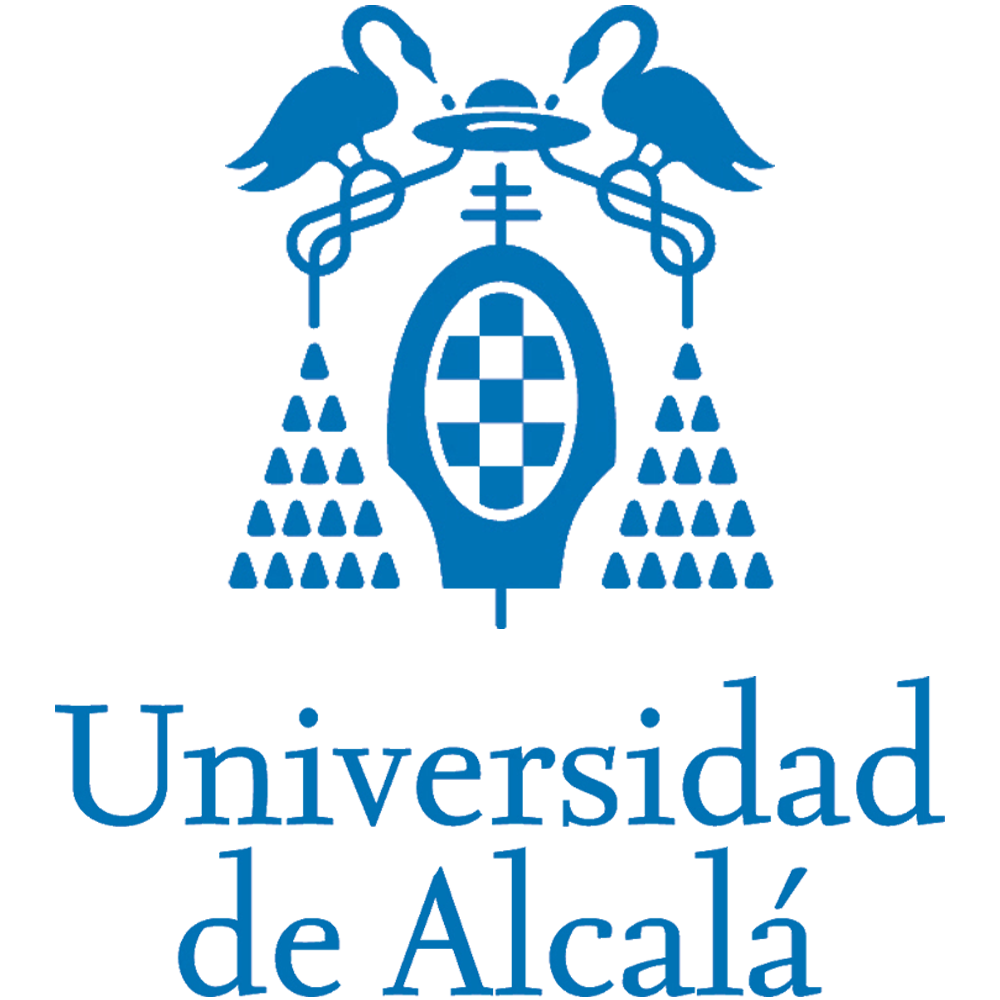
\includegraphics[width=10cm]{./image/logos/uahlogo3.png}

La migración será de la siguiente forma:

\begin{lstlisting}[language=Ruby]
class CreateOrders < ActiveRecord::Migration
  def change
    create_table :customers do |t|
      t.string :name
      t.timestamps null: false
    end
 
    create_table :orders do |t|
      t.belongs_to :customer, index: true
      t.datetime :order_date
      t.timestamps null: false
    end
  end
end
\end{lstlisting}


\myparagraph{Asociación \texttt{has\_one}}
La asociación \texttt{has\_one} es una conexión de uno-a-uno con otro modelo. Aunque parecida a la asociación anterior, ésta indica que cada instancia del modelo $\alpha$ contiene o posee una y sólo una instancia del modelo $\beta$. Para declarar dicha asociación, se procede de la siguiente forma:\footnote{Análogamente a la asociación \texttt{belongs\_to}, ésta también utiliza el singular del modelo al que se refiere.}

\begin{lstlisting}[language=Ruby]
class Supplier < ActiveRecord::Base
  has_one :account
end
\end{lstlisting}

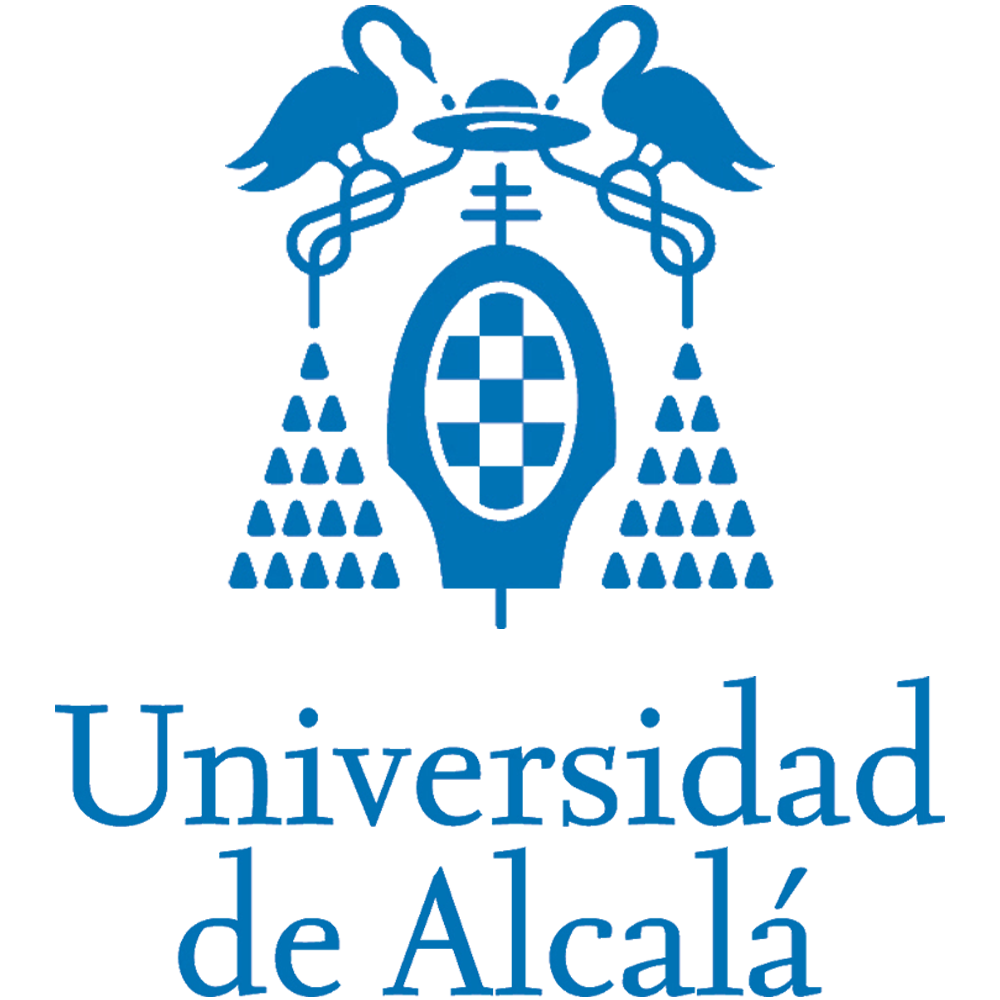
\includegraphics[width=10cm]{./image/logos/uahlogo3.png}

La migración será de la siguiente forma:

\begin{lstlisting}[language=Ruby]
class CreateSuppliers < ActiveRecord::Migration
  def change
    create_table :suppliers do |t|
      t.string :name
      t.timestamps null: false
    end
 
    create_table :accounts do |t|
      t.belongs_to :supplier, index: true
      t.string :account_number
      t.timestamps null: false
    end
  end
end
\end{lstlisting}


\myparagraph{Asociación \texttt{has\_many}}
La asociación \texttt{has\_many} indica la relación de un modelo $\alpha$ de uno-a-muchos con otro modelo $\beta$. Es común encontrar esta asociación con la relación \texttt{belongs\_to} en el otro modelo. La asociación indica que instancia del modelo tiene cero o varias instancias del otro modelo.\footnote{Se escribir nombre del modelo en forma plural en la declaración de la relación. }

\begin{lstlisting}[language=Ruby]
class Customer < ActiveRecord::Base
  has_many :orders
end
\end{lstlisting}

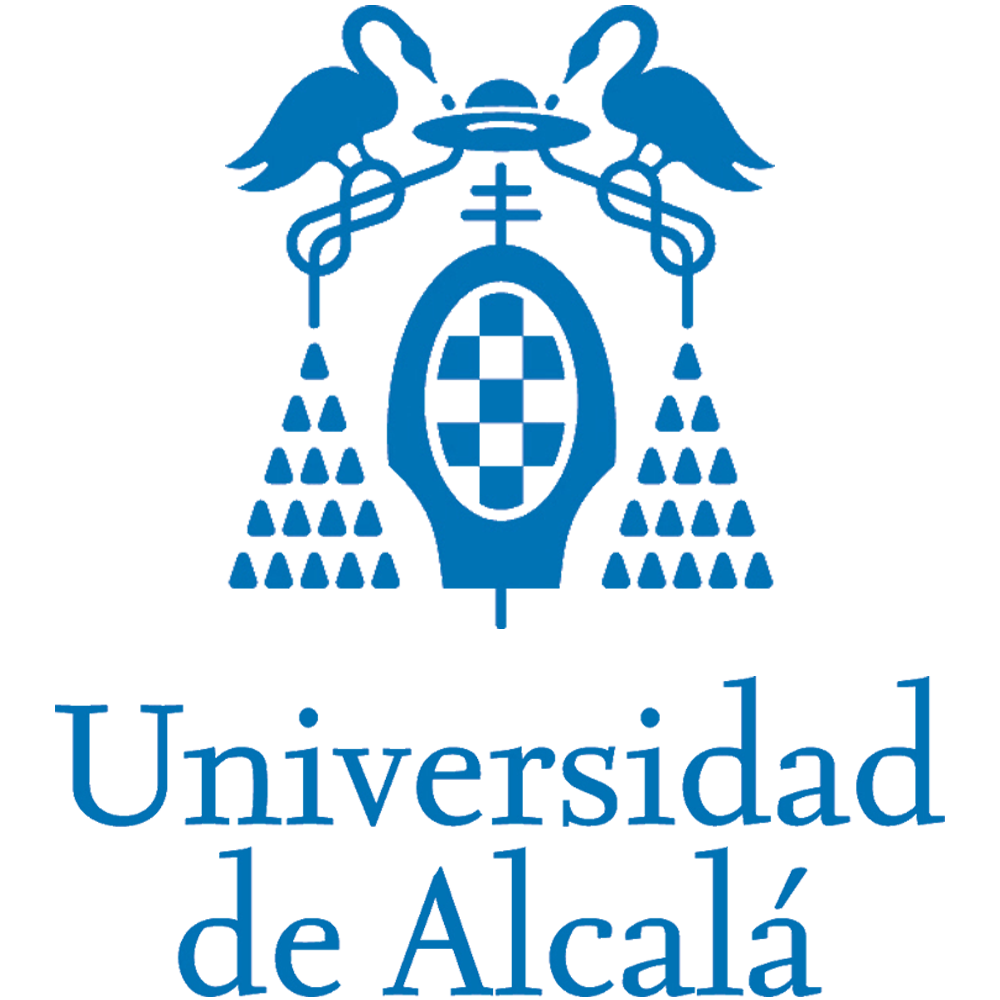
\includegraphics[width=10cm]{./image/logos/uahlogo3.png}

La migración será de la siguiente forma:

\begin{lstlisting}[language=Ruby]
class CreateCustomers < ActiveRecord::Migration
  def change
    create_table :customers do |t|
      t.string :name
      t.timestamps null: false
    end
 
    create_table :orders do |t|
      t.belongs_to :customer, index:true
      t.datetime :order_date
      t.timestamps null: false
    end
  end
end
\end{lstlisting}


\myparagraph{Asociación \texttt{has\_many :through}}
Ésta asociación es usada frecuentemente cuando se pretende establecer una relación de muchos-a-muchos con otro modelo. La relación indica que el modelo $\alpha$ de la declaración puede tener cero o varias instancias del otro modelo $\beta$ a través (\texttt{:thrrough}) de un modelo $\gamma$ intermedio.

\begin{lstlisting}[language=Ruby]
class Doctor < ActiveRecord::Base
  has_many :appointments
  has_many :patients, through: :appointments
end
 
class Appointment < ActiveRecord::Base
  belongs_to :doctor
  belongs_to :patient
end
 
class Patient < ActiveRecord::Base
  has_many :appointments
  has_many :doctors, through: :appointments
end
\end{lstlisting}

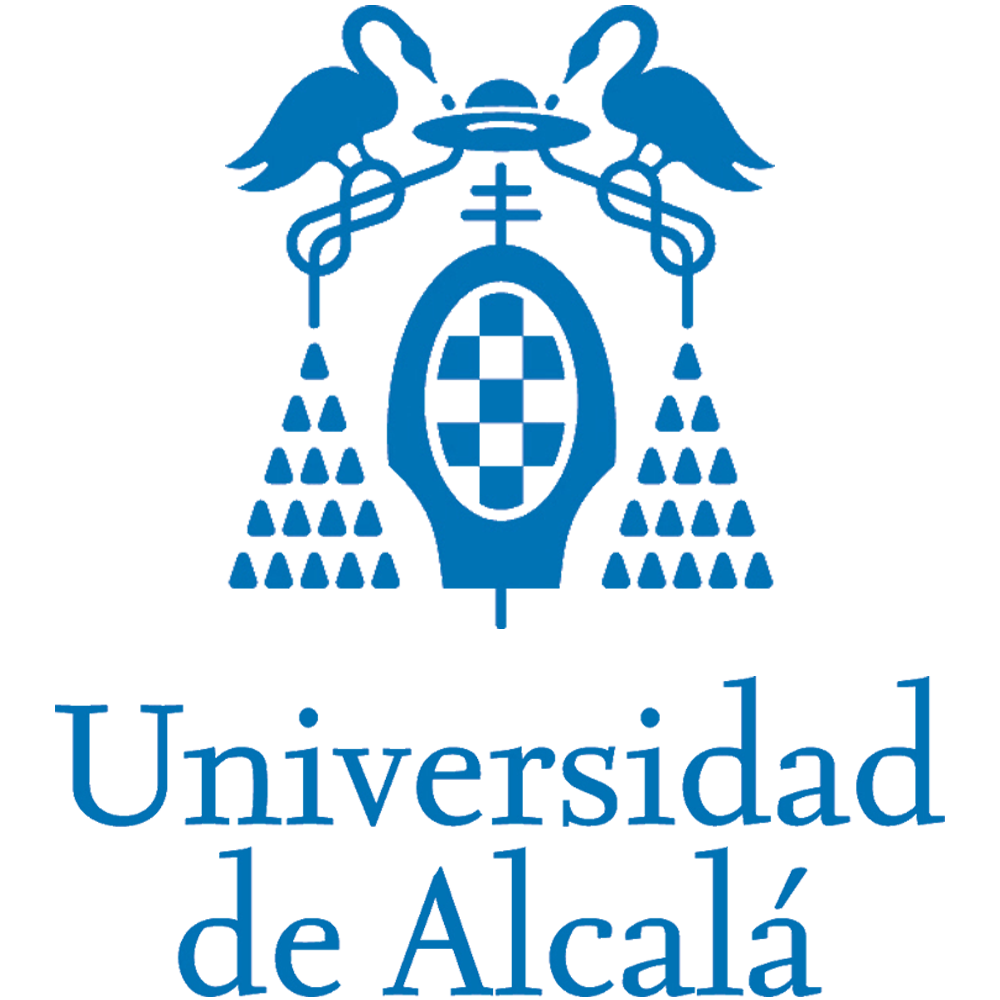
\includegraphics[width=10cm]{./image/logos/uahlogo3.png}

La migración será de la siguiente forma:

\begin{lstlisting}[language=Ruby]
class CreateAppointments < ActiveRecord::Migration
  def change
    create_table :doctors do |t|
      t.string :name
      t.timestamps null: false
    end
 
    create_table :patients do |t|
      t.string :name
      t.timestamps null: false
    end
 
    create_table :appointments do |t|
      t.belongs_to :doctor, index: true
      t.belongs_to :patient, index: true
      t.datetime :appointment_date
      t.timestamps null: false
    end
  end
end
\end{lstlisting}

Una de las grandes ventajas de esta técnica es que permite realizar la operación \textit{join} de la base de datos con una sintaxis de orientación a objetos clara.

\begin{lstlisting}[language=Ruby]
#Esta instrucción asigna una lista de pacientes a un doctor.
doctor.patients = patients
\end{lstlisting}


\myparagraph{Asociación \texttt{has\_one :through}}
La asociación \texttt{has\_one :through} establece una conexión de un modelo $\alpha$ de uno-a-uno con otro modelo $\beta$ a través de un tercer modelo $\gamma$.

\begin{lstlisting}[language=Ruby]
class Supplier < ActiveRecord::Base
  has_one :account
  has_one :account_history, through: :account
end
 
class Account < ActiveRecord::Base
  belongs_to :supplier
  has_one :account_history
end
 
class AccountHistory < ActiveRecord::Base
  belongs_to :account
end
\end{lstlisting}

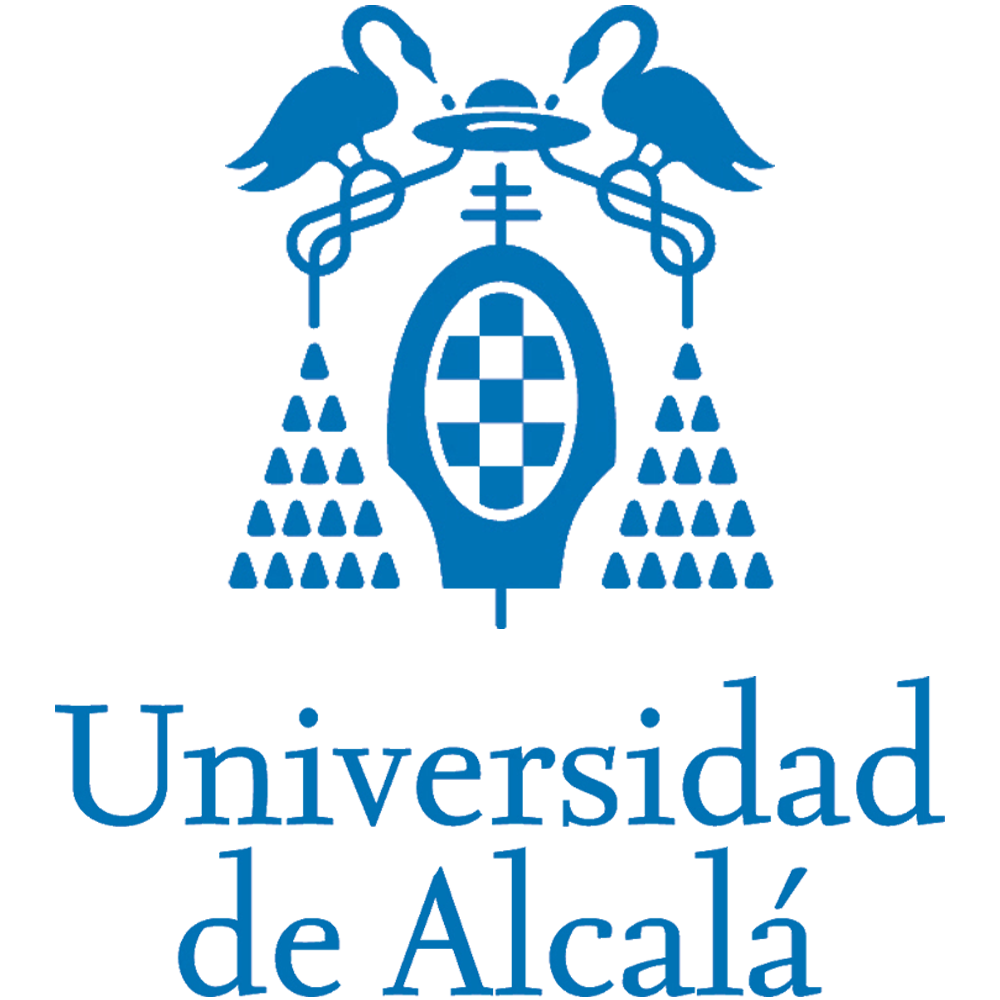
\includegraphics[width=10cm]{./image/logos/uahlogo3.png}

La migración será de la siguiente forma:

\begin{lstlisting}[language=Ruby]
class CreateAccountHistories < ActiveRecord::Migration
  def change
    create_table :suppliers do |t|
      t.string :name
      t.timestamps null: false
    end
 
    create_table :accounts do |t|
      t.belongs_to :supplier, index: true
      t.string :account_number
      t.timestamps null: false
    end
 
    create_table :account_histories do |t|
      t.belongs_to :account, index: true
      t.integer :credit_rating
      t.timestamps null: false
    end
  end
end
\end{lstlisting}


\myparagraph{Asociación \texttt{has\_and\_belongs\_to\_many}}
La asociación \texttt{has\_and\_belongs\_to\_many}, comúnmente llamada \textbf{HABTM}, crea una conexión directa de un modelo $\alpha$ y otro modelo $\beta$.

\begin{lstlisting}[language=Ruby]
class Assembly < ActiveRecord::Base
  has_and_belongs_to_many :parts
end
 
class Part < ActiveRecord::Base
  has_and_belongs_to_many :assemblies
end
\end{lstlisting}

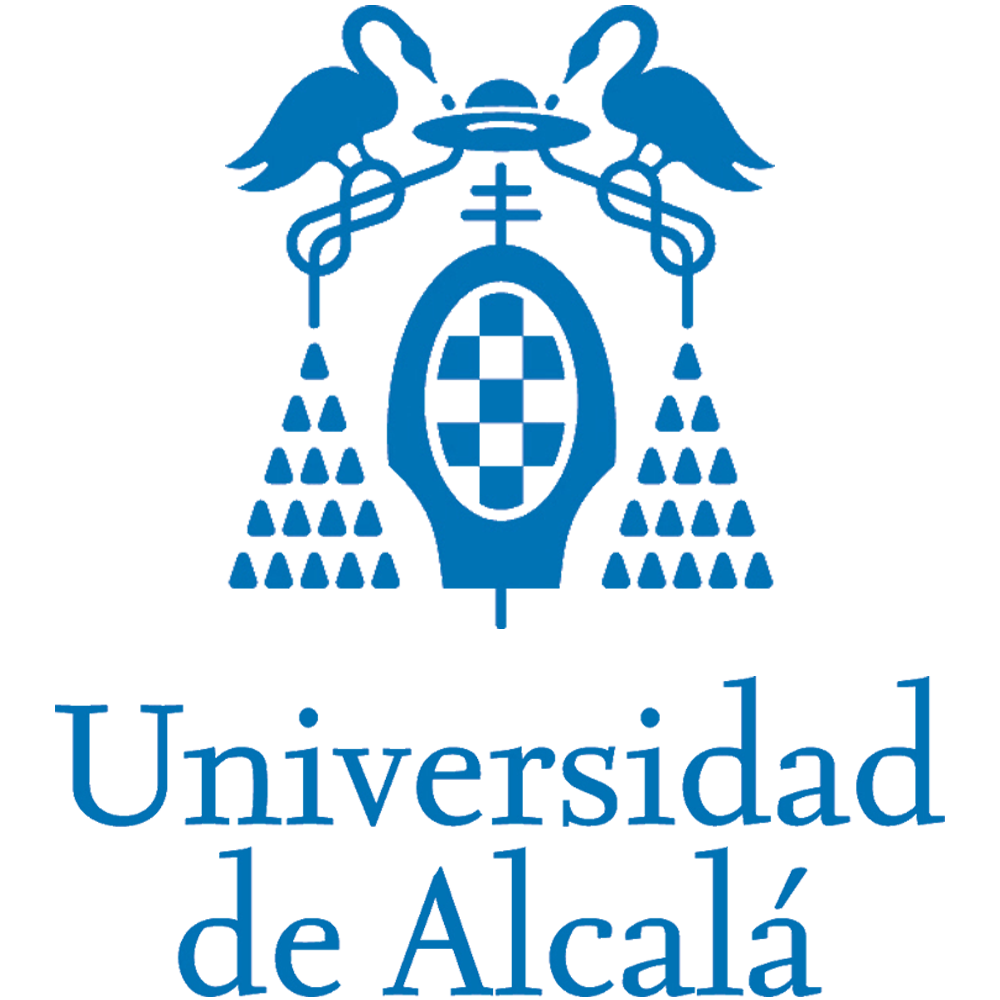
\includegraphics[width=10cm]{./image/logos/uahlogo3.png}

La migración será de la siguiente forma:

\begin{lstlisting}[language=Ruby]
class CreateAssembliesAndParts < ActiveRecord::Migration
  def change
    create_table :assemblies do |t|
      t.string :name
      t.timestamps null: false
    end
 
    create_table :parts do |t|
      t.string :part_number
      t.timestamps null: false
    end
 
    create_table :assemblies_parts, id: false do |t|
      t.belongs_to :assembly, index: true
      t.belongs_to :part, index: true
    end
  end
end
\end{lstlisting}


\myparagraph{Asociaciones polimorficas}
Gracias a las asociaciones polimorficas, es posible definir un modelo que pertenece a más de un solo modelo, con una sola asociación.

\begin{lstlisting}[language=Ruby]
class Picture < ActiveRecord::Base
  belongs_to :imageable, polymorphic: true
end
 
class Employee < ActiveRecord::Base
  has_many :pictures, as: :imageable
end
 
class Product < ActiveRecord::Base
  has_many :pictures, as: :imageable
end
\end{lstlisting}

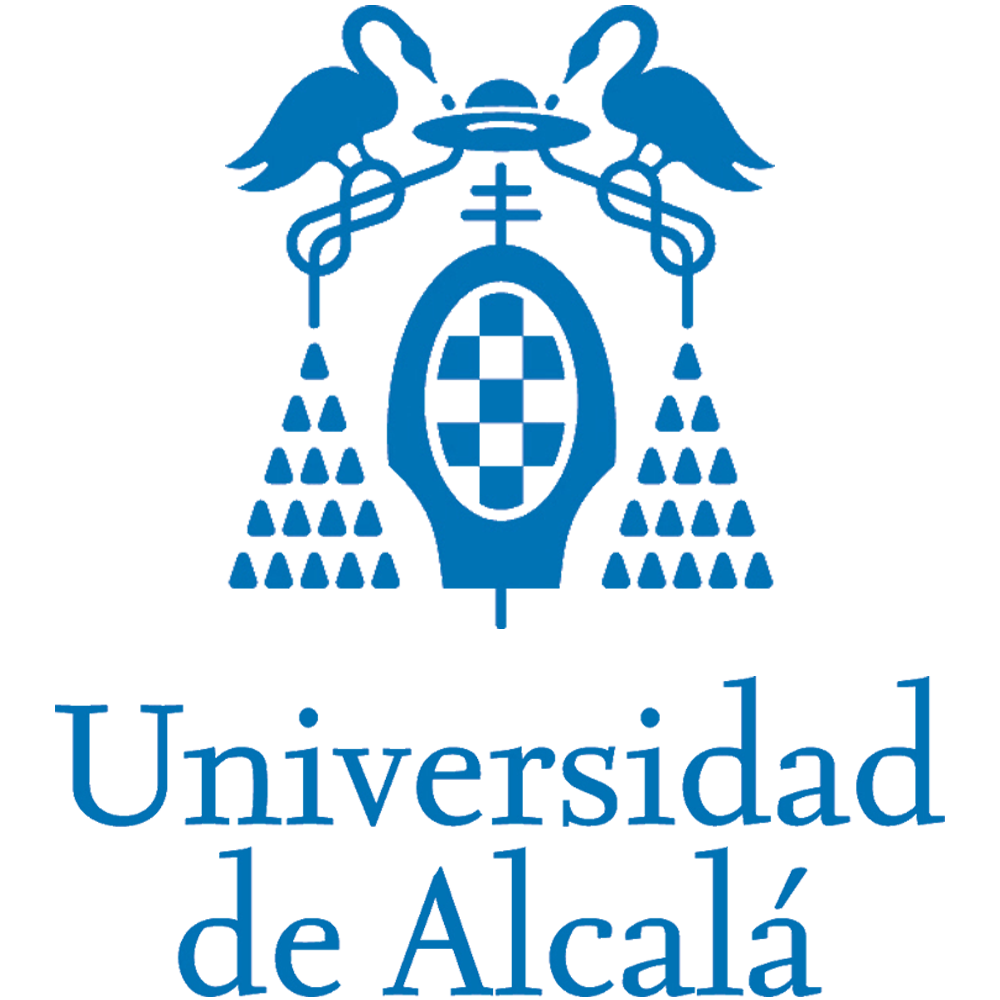
\includegraphics[width=10cm]{./image/logos/uahlogo3.png}

La migración será de la siguiente forma:

\begin{lstlisting}[language=Ruby]
class CreatePictures < ActiveRecord::Migration
  def change
    create_table :pictures do |t|
      t.string  :name
      t.integer :imageable_id
      t.string  :imageable_type
      t.timestamps null: false
    end
 
    add_index :pictures, :imageable_id
  end
end
\end{lstlisting}

Las migraciones polimorficas también pueden ser simplificadas con el método \texttt{references}.

\begin{lstlisting}[language=Ruby]
class CreatePictures < ActiveRecord::Migration
  def change
    create_table :pictures do |t|
      t.string :name
      t.references :imageable, polymorphic: true, index: true
      t.timestamps null: false
    end
  end
end
\end{lstlisting}



\subsection{Interfaz de consultas}
Active Record ejecuta consultas en la base de datos a través de su interfaz. El interfaz es compatible con la mayor parte de las bases de datos (MySQL, PostgreSQL, y SQLite), por lo que independientemente que se utilice, Active Record ejecutará las consultas, siempre, de la misma forma.

